\documentclass[a4paper, 12pt, svgnames]{article}

\usepackage{preambule}

\title{Variabilités intrinsèques des SNe Ia et leurs conséquences sur les
paramètres cosmologiques}

\fancyhead[L]{\scriptsize \textsc{Variabilités intrinsèques des SNe Ia}}

\begin{document}

\thispagestyle{empty}
\noindent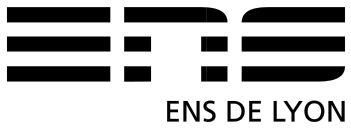
\includegraphics[height=2cm]{General_figures/logoens.png} \hfill

\includegraphics[height=2cm]{General_figures/logoucbl.png} \hfill

\includegraphics[height=2cm]{General_figures/logounivlyon.png}\vfill

\noindent\begin{tabularx}{\linewidth+27pt}{@{} l X r @{} }
{\textsc{Master Science de la matière}} & & Année 2018--2019\hspace*{1cm}\\
{\textit{École Normale Supérieure de Lyon}} & & \textsc{Nicolas} Nora\hspace*{1cm}\\
{\textit{Université Claude Bernard Lyon I}} & & M2 Physique\hspace*{1cm}
\end{tabularx}

\begin{center}\vfill\hrule\vspace*{8pt}

\textbf{\huge Variabilités intrinsèques des SNe Ia et leurs conséquences sur les
paramètres cosmologiques}\\

\hrule\vfill

\parbox{15cm}{\small\textbf{Résumé}:
L'étude des supernovae de type Ia a de nombreuses utilités en physique. Elle
sert notamment à la détermination de paramètres cosmologiques, comme la
constante de Hubble ou le paramètre d'état de l'énergie noire. Afin d'améliorer
la précision et la justesse des mesures existantes, les incertitudes
statistiques et systématiques doivent être traitées correctement. Si l'ajout de
données permet de réduire les incertitudes statistiques, il n'y a que l'étude du
comportement physique des supernovae qui permet de réduire les incertitudes
systématiques. Dans ce rapport, nous discutons comment l'établissement de lois
d'évolution du paramètre de durée d'explosion d'une supernova en fonction du
redshift permettrait d'atteindre ce but.}\vspace{0.5cm}

\parbox{15cm}{\small\textbf{Mots-clés}:
Cosmologie, supernovae}\vspace{0.5cm}

\parbox{15cm}{Stage supervisé par:\\
\textbf{\textsc{RIGAULT} Mickaël}, Chercheur\\
\href{mailto:rigault@ipnl.in2p3.fr}{rigault@ipnl.in2p3.fr}\\
\href{https://www.ipnl.in2p3.fr/perso/rigault/}{Site personnel}\bigbreak
Institut de Physique des Deux Infinis\\
{\textit{Université Lyon 1\\4 rue Enrico Fermi -- bâtiment Dirac\\
69622 Villeurbanne Cedex}}\\
\url{https://www.ipnl.in2p3.fr}}\vspace{.5cm}\vfill


\includegraphics[width=.3\textwidth]{General_figures/IP2I.png}
\end{center}\vfill \hfill \today
\newpage
\thispagestyle{empty}
\setcounter{page}{0}

\appsec{Remerciements}{sec:ack}

Je tiens à remercier toutes les personnes qui ont contribué, de près ou de loin,
à la réalisation de ce stage et de ce rapport de stage. En premier lieu, bien
évidemment, je remercie Mickaël \bsc{Rigault} pour son encadrement sans faille

\tableofcontents
\newpage

\section{Introduction}\label{sec:int}
\subsection{Le domaine de recherche}

La combinaison des observations et des prédictions théoriques du modèle du Big
Band indiquent que l'univers est en expansion. Lors de la découverte de cette
expansion, on pensait qu'elle devrait ralentir sous l'effet de la gravitation.
Cependant, l'utilisation des supernovae de type Ia (SNe Ia) par \bsc{Perlmutter
et al.}~\cite{perlmutter_measurements_1999}, \bsc{Riess et al.}
~\cite{riess_observational_1998} et \bsc{Schmidt et al.}
~\cite{schmidt_high-z_1998} a permis de mettre en évidence l'expansion
accélérée de l'Univers, découverte pour laquelle ils ont eu le prix Nobel de
physique de 2011. Il y aurait ainsi un phénomène allant à l'encontre des
effets gravitationnels, phénomène qui a été nommé « énergie noire » : la
cosmologie moderne vise entre aux à mieux comprendre la nature de cette énergie,
sa proportion dans l'Univers et les lois physiques auxquelles elle obéit.

\begin{itemize}
    \item Tension sur $H_0$? \bsc{Riess et al.} 2016 donne des valeurs en intro
\end{itemize}

\subsection{Diagramme de Hubble}
Cette découverte a été effectuée par l'utilisation des mesures des flux lumineux
de supernovae, exprimés en magnitude qui en est le logarithme. Le flux est relié
à la luminosité $L$ d'une source lumineuse et à la distance $d_L$ entre la source
et le point d'observation par la relation

\begin{equation}
    F = \frac{L}{4\pi d_L²}
\end{equation}

et la magnitude apparente $m$ est reliée au flux reçu par la relation

\begin{equation}
    m - m_0 = -2.5\log\LR{F}{F_0} = -2.5\log\LR{L}{4\pi d_L²} + C
\end{equation}

avec $F_0$ le flux d'une étoile de référence. Cette définition de la magnitude
dépend donc de la distance ; on définit alors une magnitude \textit{absolue}
traduisant la luminosité intrinsèque du corps observé : c'est la magnitude
apparente que percevrait un observateur situé à une distance de $\SI{10}{pc}$ de
la source, autrement dit

\begin{equation}
    M = -2.5\log\LR{L}{4\pi\LF{\SI{10}{pc}}²} + C
\end{equation}

On peut alors définir le \textit{module de distance} $\m$ défini par

\begin{equation}
    \m \equiv m - M = 5\log(d_L) - 5
\end{equation}

avec $d_L$ en parsec. Or, en considérant un univers plat homogène et isotrope,
l'équation de \bsc{Friedmann}-\bsc{Lemaître} mène à une expression de $d_L$
dépendant des paramètres cosmologiques d'après la relation

\begin{equation}\label{dL}
    d_L = \LF{1 + z} \times c \LF{ \int_0^z \d z' \left[ \O_R
    \LF{1 + z'}⁴ + \O_M \LF{1 + z'}³ + \O_{\L} \right]^{-1/2}}
\end{equation}

avec $\O_R$ la densité d'énergie de rayonnement, $\O_M$ la densité d'énergie de
matière, et $\O_\L$ la densité d'énergie noire. Elles sont reliées par la
relation

\begin{equation}
    1 = \O_R + \O_M + \O_\L
\end{equation}

pour un univers plat.

\textcolor{orange}{Rajouter développement en annexe ?}

Ainsi, le module de distance $\m$ permet de de déterminer $d_L$ \textit{via} la
mesure de la magnitude apparente $m$, si la magnitude absolue $M$ est connue.
Les SNe Ia sont utilisées pour leur magnitude absolue \textit{a priori}
standard, ce qui leur a valu le nom de \textit{chandelles standards}.

En réalité, il existe une dispersion naturelle d'environ 40\% des magnitudes
absolues des SNe Ia. Cette dispersion implique une imprécision sur la valeur de
la distance déduite par la mesure de magnitude apparente de 20\%.

%, comme le
%montre la figure ci-après :
%
%\begin{figure}[htbp!]
%    \centering
%    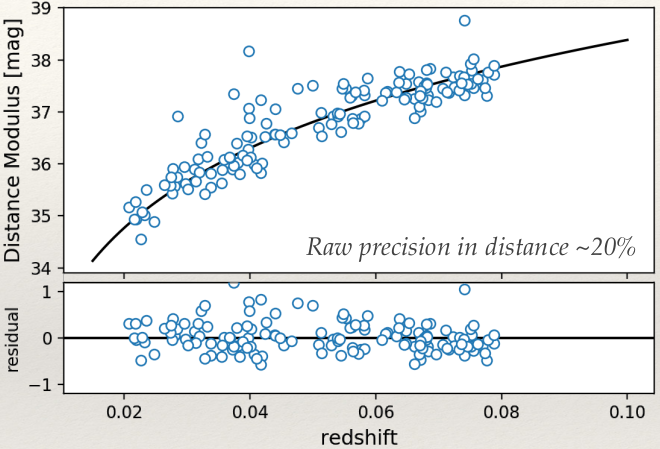
\includegraphics[width = .5\linewidth]{Rapport_figures/disp_40.png}
%    \captionsetup{justification=centering}
%    \caption{Effet de la dispersion naturelle de la magnitude absolue
%    des SNe Ia sur la mesure du module de distance par rapport à l'évolution
%attendue (en noir).}
%    \label{disp_40}
%\end{figure}

\begin{itemize}
    \item Mesure de magnitude, équations ;
    \item Dispersion naturelle, imprécision.
\end{itemize}

\subsection{Les SNe Ia}

Si les SNe Ia sont considérées comme des chandelles standards, c'est parce
qu'elles obéissent au même mécanisme d'explosion. Bien qu'il soit encore mal
compris, on sait qu'il résulte de l'augmentation de la masse de naines
blanches, des étoiles inertes très denses, qui mènerait à une explosion
thermonucléaire lorsqu'elles atteignent la masse critique de \bsc{Chandrasekhar}
de \SI{1.4}{M_\odot}. Cette augmentation peut suivre de l'accrétion d'un
compagnon qui est généralement une géante rouge, ou par fusion de deux naines
blanches.

Elles sont beaucoup étudiées en cosmologie de fait de leur forte luminosité
permettant une mesure de magnitude jusqu'à des redshifts de l'ordre de $z
\approx 1$, ce qui équivaut à une analyse des propriétés cosmologiques de
l'Univers quand il était de la moitié de son âge actuel. Elles sont notamment
les meilleures candidates pour les études à bas redshift, leur luminosité (sur
une courte période) pouvant dépasser celle de leur galaxie hôte contenant des
centaines de milliards d'étoiles,  et qui, d'après l'équation \ref{dL}, est la
zone d'Univers où le paramètre d'énergie noire domine (pour $z \leq 1$, c'est le
terme en $\O_\L$ qui domine étant donné la puissance $-1/2$ sur le crochet). Un
des buts de l'utilisation des SNe Ia en cosmologie est de mieux comprendre le
comportement de cette énergie noire, sa densité précise et l'évolution de sa
densité.

\begin{itemize}
    \item Spécificité astrophysique ;
    \item Pertinence cosmologique.
\end{itemize}

\subsection{Courbes de lumière}
Pour réaliser les mesures de magnitudes, une seule acquisition n'est pas
suffisante. On s'intéresse à l'évolution de la luminosité d'une supernova à
partir du moment de son explosion. Cette analyse permet de définir plusieurs
paramètres (cf. figure \ref{lightcurves}) \textcolor{orange}{Rajouter
références !}

\begin{enumerate}
    \item Le paramètre de \textit{color}, défini par la différence de magnitude
        au maximum d'émission entre les bandes vertes et bleues ;
    \item Le paramètre de \textit{stretch}, définissant la durée de l'explosion
        de la supernova ; il s'apparente à la largeur à mi-hauteur d'un
        gaussienne mais pour une distribution non symétrique.
\end{enumerate}

\begin{figure}[htbp!]
    \centering
    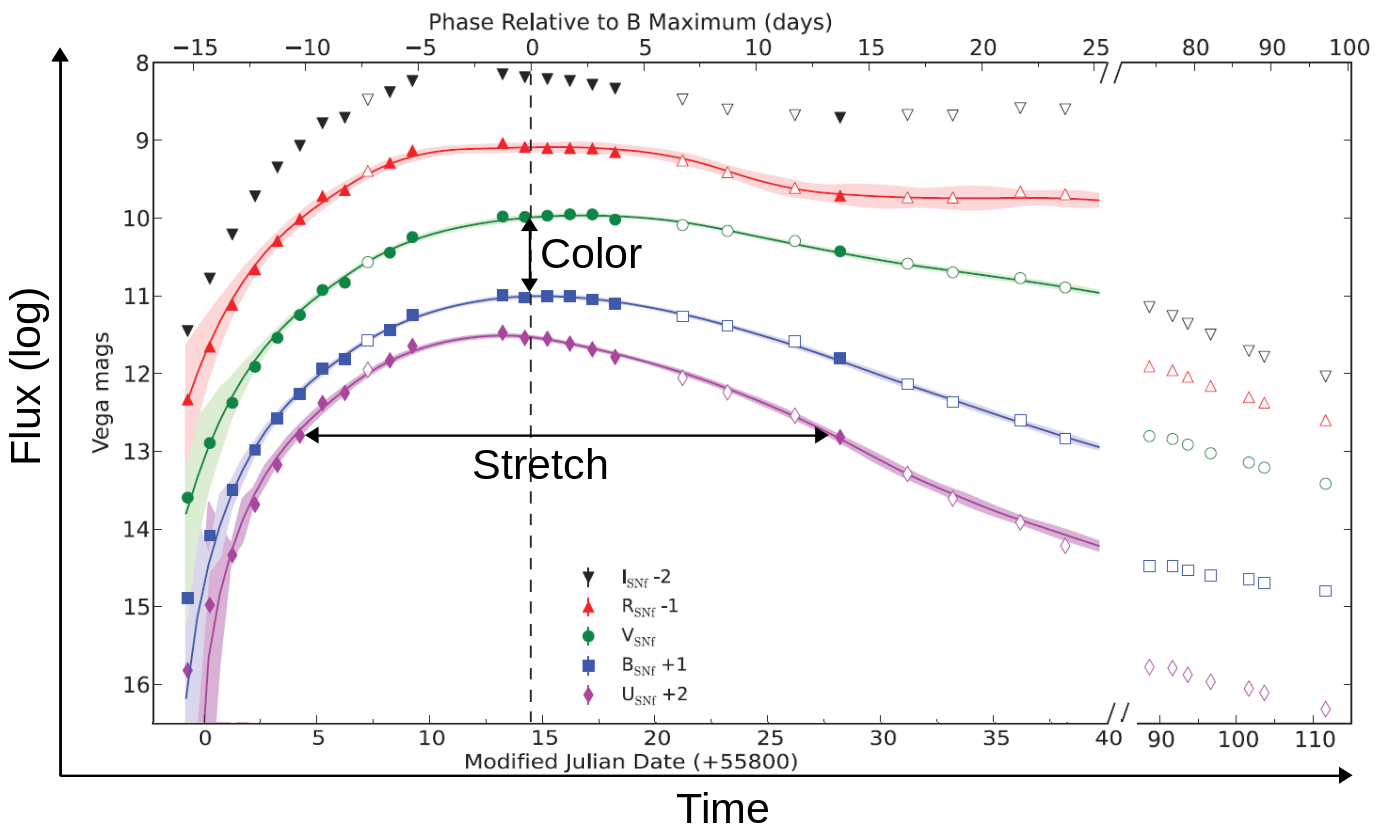
\includegraphics[width=.5\linewidth]{Rapport_figures/lightcurve.png}
    \captionsetup{justification=centering}
    \caption{Exemple de courbe de lumière d'une supernova depuis son explosion
    pour différentes longueurs d'ondes. On peut y définir un paramètre de
couleur et un paramètre de \textit{stretch} qui estime la durée d'explosion de
ladite SNe Ia.}
    \label{lightcurves}
\end{figure}

La définition de ces paramètres n'est pas anodine : il a en effet été montré
qu'une corrélation forte existe entre la valeur de ces paramètres et la
magnitude absolue $M_B{}^{\text{max}}$ d'une supernova. Notamment, les SNe Ia
avec une grande durée d'explosion (grand stretch) on une luminosité intrinsèque
plus grande (relation appelée "brighter-slower"), et que les SNe Ia les plus
bleues sont également plus lumineuses (relation "brighter-bluer"). On peut voir
ces corrélations figure \ref{brighter_slower_bluer}.

\begin{figure}[htbp!]
    \centering
    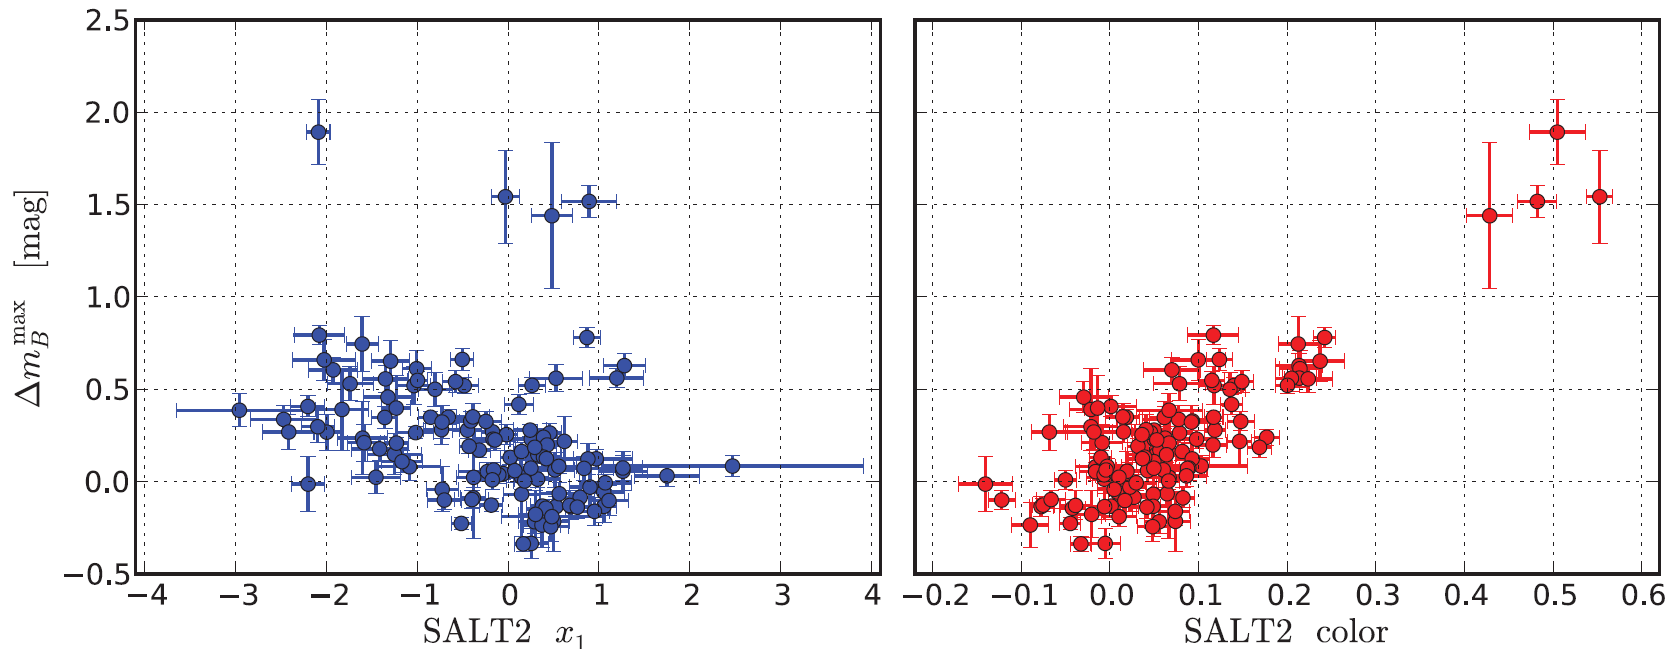
\includegraphics[width=.7\linewidth]{Rapport_figures/disp_x1_c.PNG}
    \captionsetup{justification=centering}
    \caption{Corrélations entre la différence de luminosité maximale d'une
    supernova dans le bleu et les paramètres de stretch (« $x_1$ ») et de
couleur (« color ») d'après l'algorithme SALT2.}
    \label{brighter_slower_bluer}
\end{figure}

On peut alors inclure ces relations linéaires dans l'expression de la magnitude
absolue, \textit{via} la relation

\begin{equation}
    \D M_B{}^{\text{corr}} \equiv \LF{M_B{}^{\text{max}} - M_B{}^0} + \LF{\a x_1
    - \b c}
\end{equation}

où $\a$ est le coefficient du stretch, et $\b$ celui de la couleur, tous les
deux positifs, avec $M_B{}^0$ la magnitude moyenne des SNe Ia. Tous ces
paramètres sont ajustés simultaniément sur l'ensemble des données disponibles.
Ces relations supplémentaires permettent de réduire l'incertitude sur le
paramètre de magnitude absolue, et d'avoir une détermination de la distance dont
l'erreur est diminuée à 8\% (cf figure \ref{disp_20}) \textit{via} la relation

\begin{equation}
    \m = m - M +\a x_1 - \b c
\end{equation}

\begin{figure}[htbp!]
    \centering
    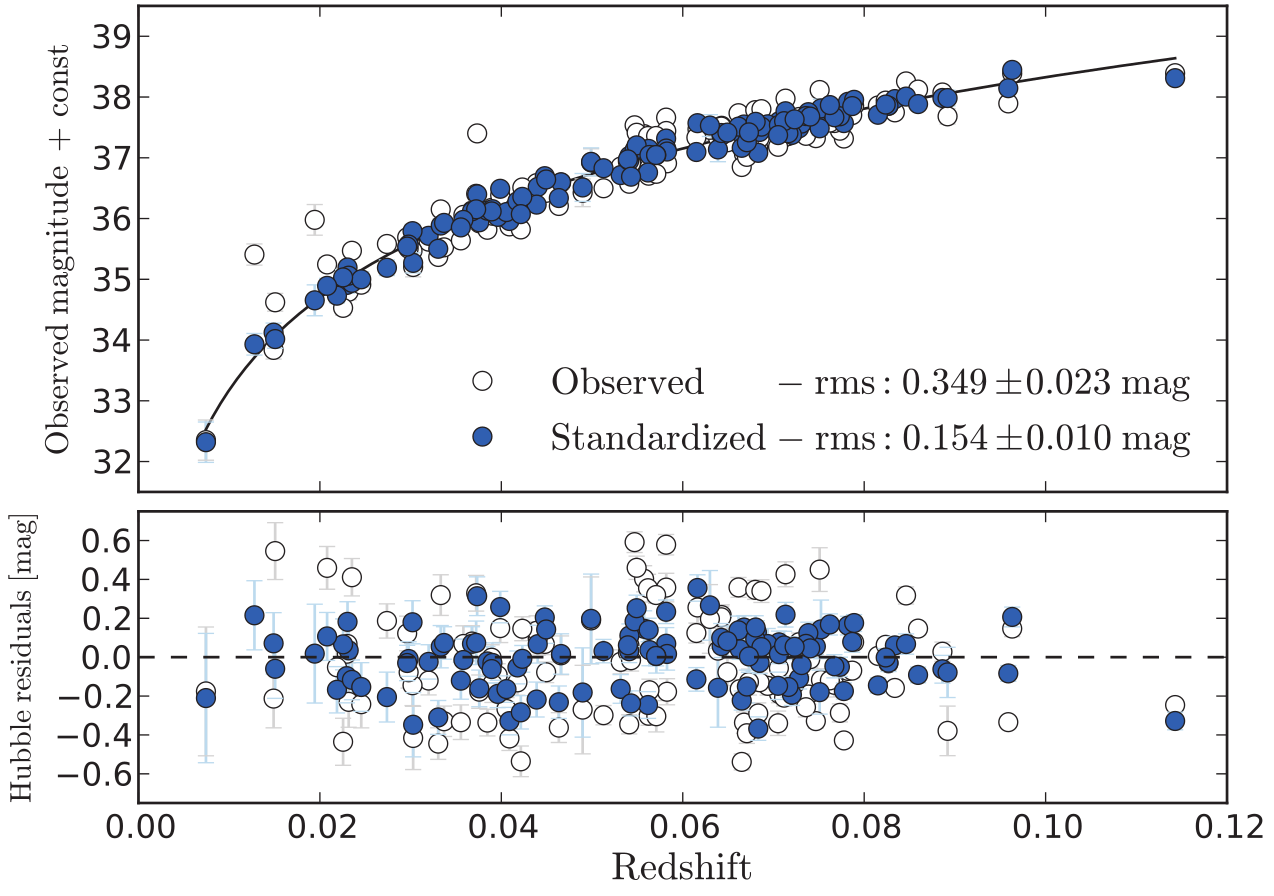
\includegraphics[width=.5\linewidth]{Rapport_figures/disp_beau.png}
    \captionsetup{justification=centering}
    \caption{Diagramme de Hubble avec, en haut, la magnitude apparente avant et
        après le processus de standardisation, qui consiste à inclure les
        corrélations entre la magnitude absolue et les paramètres de stretch et
        de couleur, respectivement en blanc et en bleu. En bas, on a le
        \textit{résidu} ne montrant que la dispersion autour de la courbe noire,
        indiquant l'évolution de la luminosité prédite par la loi de Hubble.}
    \label{disp_20}
\end{figure}

L'utilisation de cette relation a alors permis d'améliorer la précision des
mesures de distance, et ainsi discriminer différentes valeurs possibles pour les
paramètres cosmologiques : cela a mené à la découverte de l'expansion accélérée
de l'Univers \textit{via} une valeur non-nulle de $\O_\L$ pour laquelle un prix
Nobel a été descerné. Avant cette étude, l'évolution attendue du module de
distance des SNe Ia était indiqué par la courbe grise dans la figure
\ref{hub_acc_exp}.

\begin{figure}[htbp!]
    \centering
    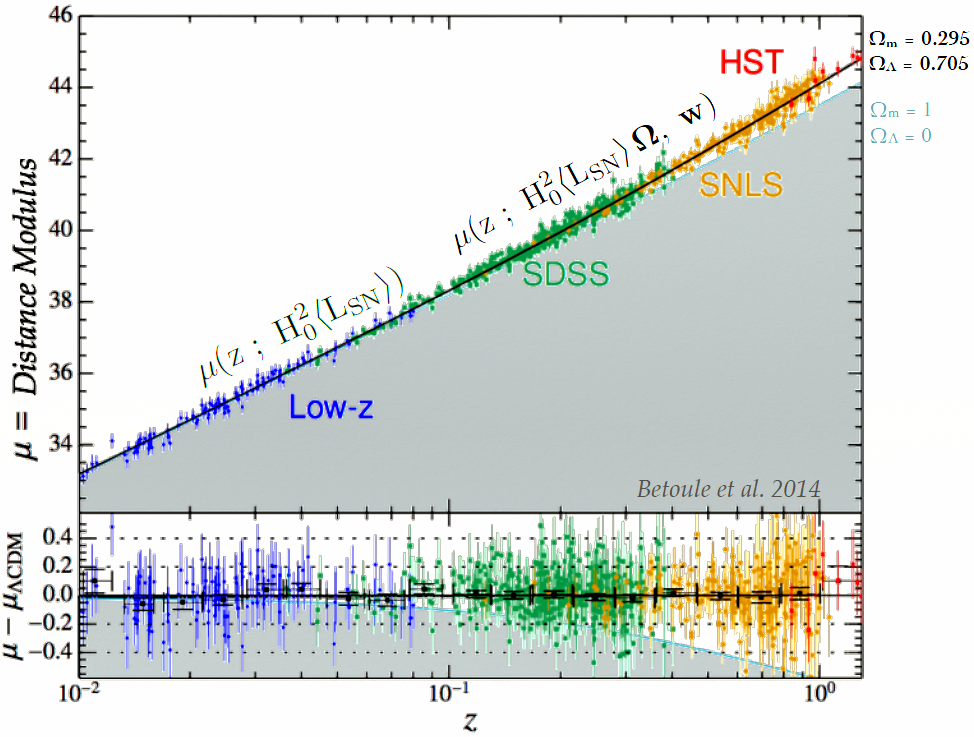
\includegraphics[width=.5\linewidth]{Rapport_figures/bet_al_2.PNG}
    \captionsetup{justification=centering}
    \caption{Diagramme de Hubble actuel (en couleurs, une par échantillon
             d'observation) comparé au diagramme de Hubble avant la découverte 
             de l'expansion accélérée de l'Univers.}
    \label{hub_acc_exp}
\end{figure}

\begin{itemize}
    \item Définitions ;
    \item Relations empiriques, équation corrigée.
\end{itemize}

\subsection{Incertitudes systématiques}

Cette avancée monumentale dans la cosmologie a pu montrer la puissance des SNe
Ia dans la détermination de paramètres cosmologiques. Depuis cette découverte,
qui ne se basait que sur une centaine de données de SNe Ia, plus de données ont
été accumulées, et la précision sur les mesures de $\O_M$ et $\O_\L$ s'est
améliorée. Cependant, sur la totalité de l'incertitude sur ces paramètres, la
part des incertitudes systématiques est très importante. C'est non seulement une
limitation à la précision des mesures, mais également un danger pour la justesse
de celles-ci. Par exemple, dans le but d’étudier l’énergie noire, et notamment
son paramètre d’état $\w$ qui devrait être de $-1$ pour correspondre à un fluide
de pression négative et sa dérivée $\w_a$ qui traduit l’évolution de ce
comportement au cours du temps, il convient de tester leur concordance avec
différents modèles cosmologiques. Il a été montré que si les erreurs
systématiques ne sont pas prises en compte et qu'on les considère comme
négligeable devant les incertitudes statistiques, l'ajout de nouvelles données
(qui est le but de la collaboration LSST qui amènera environ 100 000 données de
SNe Ia à commencer dans 3 ans) nous mènerait forcément à un résultat éloigné du
modèle que l'on souhaite tester (cf. figure \ref{err_syst}).

\begin{figure}[htbp!]
    \centering
    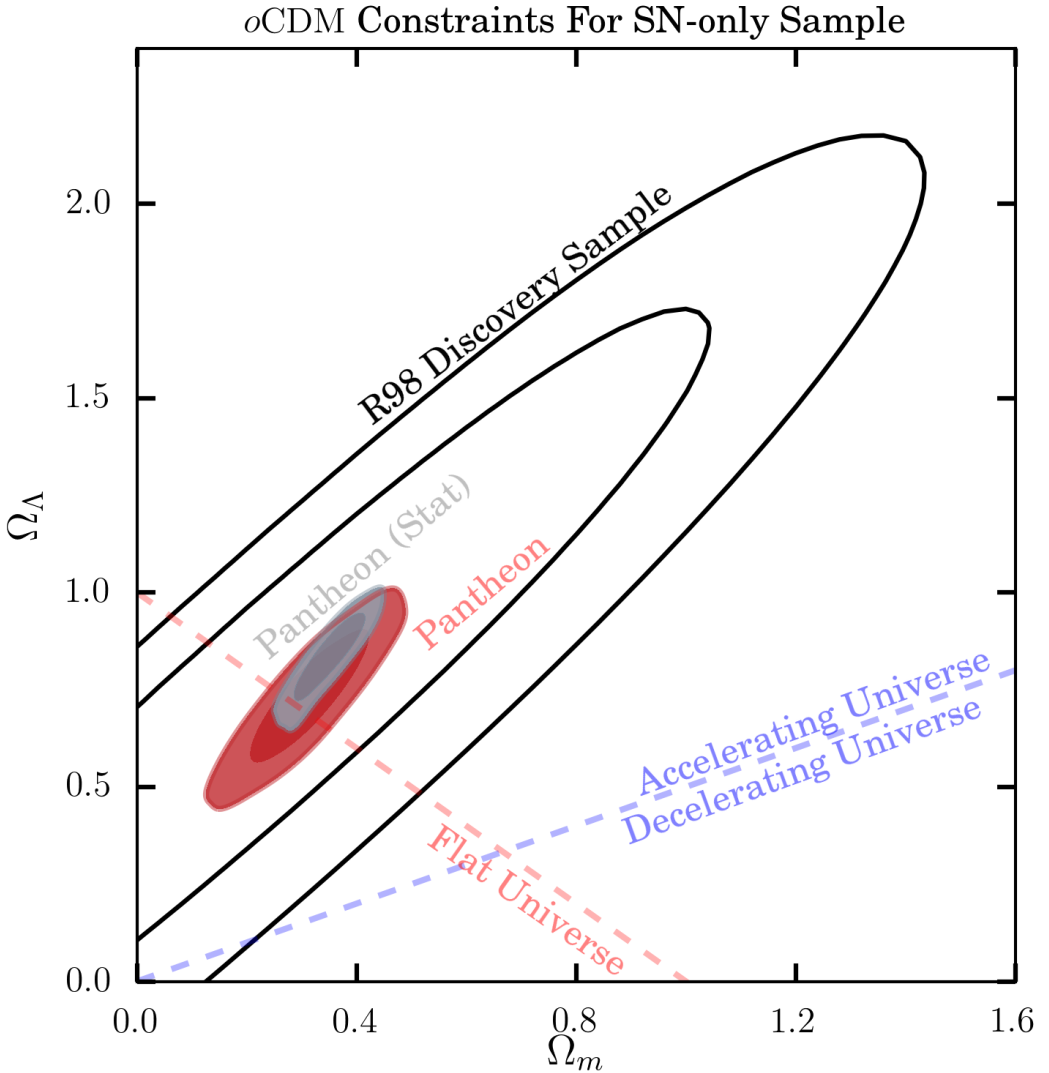
\includegraphics[width=.5\linewidth]{Rapport_figures/scolnic_syst.png}
    \captionsetup{justification=centering}
    \caption{\textit{Contour plot} indiquant la précision à 68 et 90\% de la
    mesure des paramètres $\O_M$ et $\O_\L$ pour la découverte historique de
    \bsc{Riess et. al} (R98, en blanc) se basant sur 100 données de SNe Ia, et
    pour les échantillons actuels utilisant environ 1000 SNe Ia (en rouge). En
    gris est indiqué la part des incertitudes systématiques à l'incertitude
    totale. \cite{scolnic_complete_2018}}
    \label{scolnic_syst}
\end{figure}

\begin{figure}[htbp!]
    \centering
    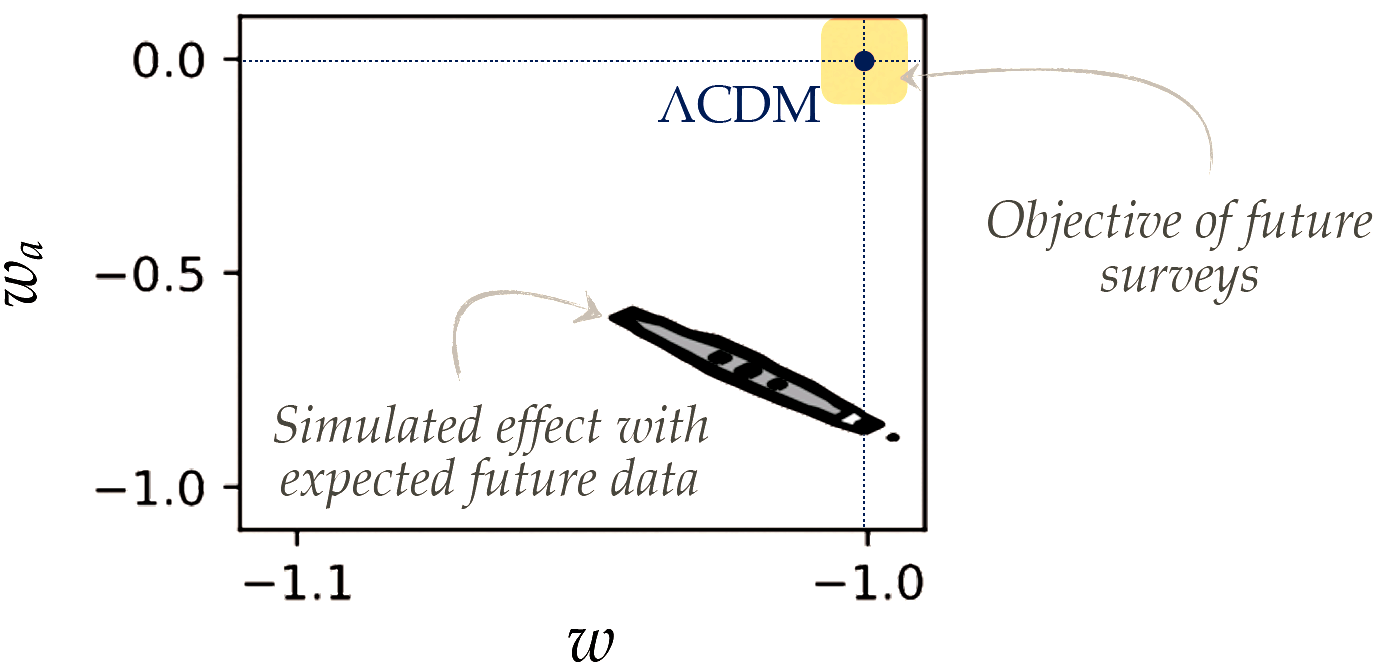
\includegraphics[width=.5\linewidth]{Rapport_figures/error.PNG}
    \captionsetup{justification=centering}
    \caption{Erreur attendue sur la mesure de $\w$ et $\w_a$ en ne considérant
    que la réduction des erreurs statistiques sans prendre en compte les erreurs
    systématiques.}
    \label{err_syst}
\end{figure}

Ainsi, si l'ajout de données permet de réduire
les incertitudes statistiques, il paraît nécessaire de travailler sur la
physique à l'origine de ces variations de magnitudes absolues pour pouvoir, dans
l'idéal, réaliser le même travail qui a été fait avec le stretch et la couleur
mais pour d'autres paramètres. C'est l'objet de ce stage et de la thèse qui en
découle.

\begin{itemize}
    \item Importance dans les mesures actuelles ;
    \item Importance dans les mesures futures.
\end{itemize}

\subsection{Problème du progéniteur}
\begin{itemize}
    \item Progéniteur inconnus :
    \item L moyennes différentes avec $z$ ou échantillon ;
    \item Évolution du \textit{lsSFR}.
\end{itemize}

Parler du fait que le code est sur GitHub, et faire des références dans la
suite.

\section{Construction d'un échantillon complet}
\subsection{Effets de sélection}
\begin{itemize}
    \item Histogramme échantillons ;
    \item Rappel relation \textcolor{red}{brighter-slower} et conclusion.
\end{itemize}

\subsection{Méthode de détermination}
\begin{itemize}
    \item Modèle d'évolution ;
    \item Statistique poissonienne, itérations pour chaque échantillon.
\end{itemize}

\section{Modèle d'évolution}
\subsection{Origine du modèle}
\begin{itemize}
    \item Données \textcolor{orange}{SNF} ;
    \item Définition jeune/vieille d'après \bsc{Rigault et al.} 2018
\end{itemize}

\subsection{Implémentation aux échantillons}
\begin{itemize}
    \item Concordance avec \textcolor{orange}{SNF} seulement
    \item Modèle \textcolor{orange}{SNF} sur toutes les données
\end{itemize}

\subsection{Modifications et comparaisons}
\begin{itemize}
    \item Modification du modèle ;
    \item Implémentation d'autres modèles et résultats
\end{itemize}

\section{Conclusion}
Conclusion

\bibliographystyle{unsrt}
\bibliography{VIDSTIA}
\addcontentsline{toc}{section}{Bibliographie}

\end{document}
